\documentclass[10pt,a4paper]{article}
\usepackage{iftex}
\ifPDFTeX
  \usepackage[T1]{fontenc}
  \usepackage[utf8]{inputenc}
\else
  \usepackage{fontspec}
\fi
\usepackage[margin=20mm]{geometry}
\usepackage{booktabs,longtable,array}
\usepackage{tikz,pgfplots}
\usetikzlibrary{arrows.meta,positioning}
\pgfplotsset{compat=1.18}
\usepackage{hyperref}
\hypersetup{hidelinks}
\setlength{\emergencystretch}{3em}
\author{FrameSIM export}
\date{}
\title{FrameSIM: fluxo da simulação e das avaliações}
\begin{document}
\maketitle
Este diagrama descreve o processo implementado, não uma execução nem validação empírica. Os provedores são opcionais; chamadas remotas dependem da configuração e do orçamento autorizado.
\clearpage
\section*{Fluxograma}
\begin{center}
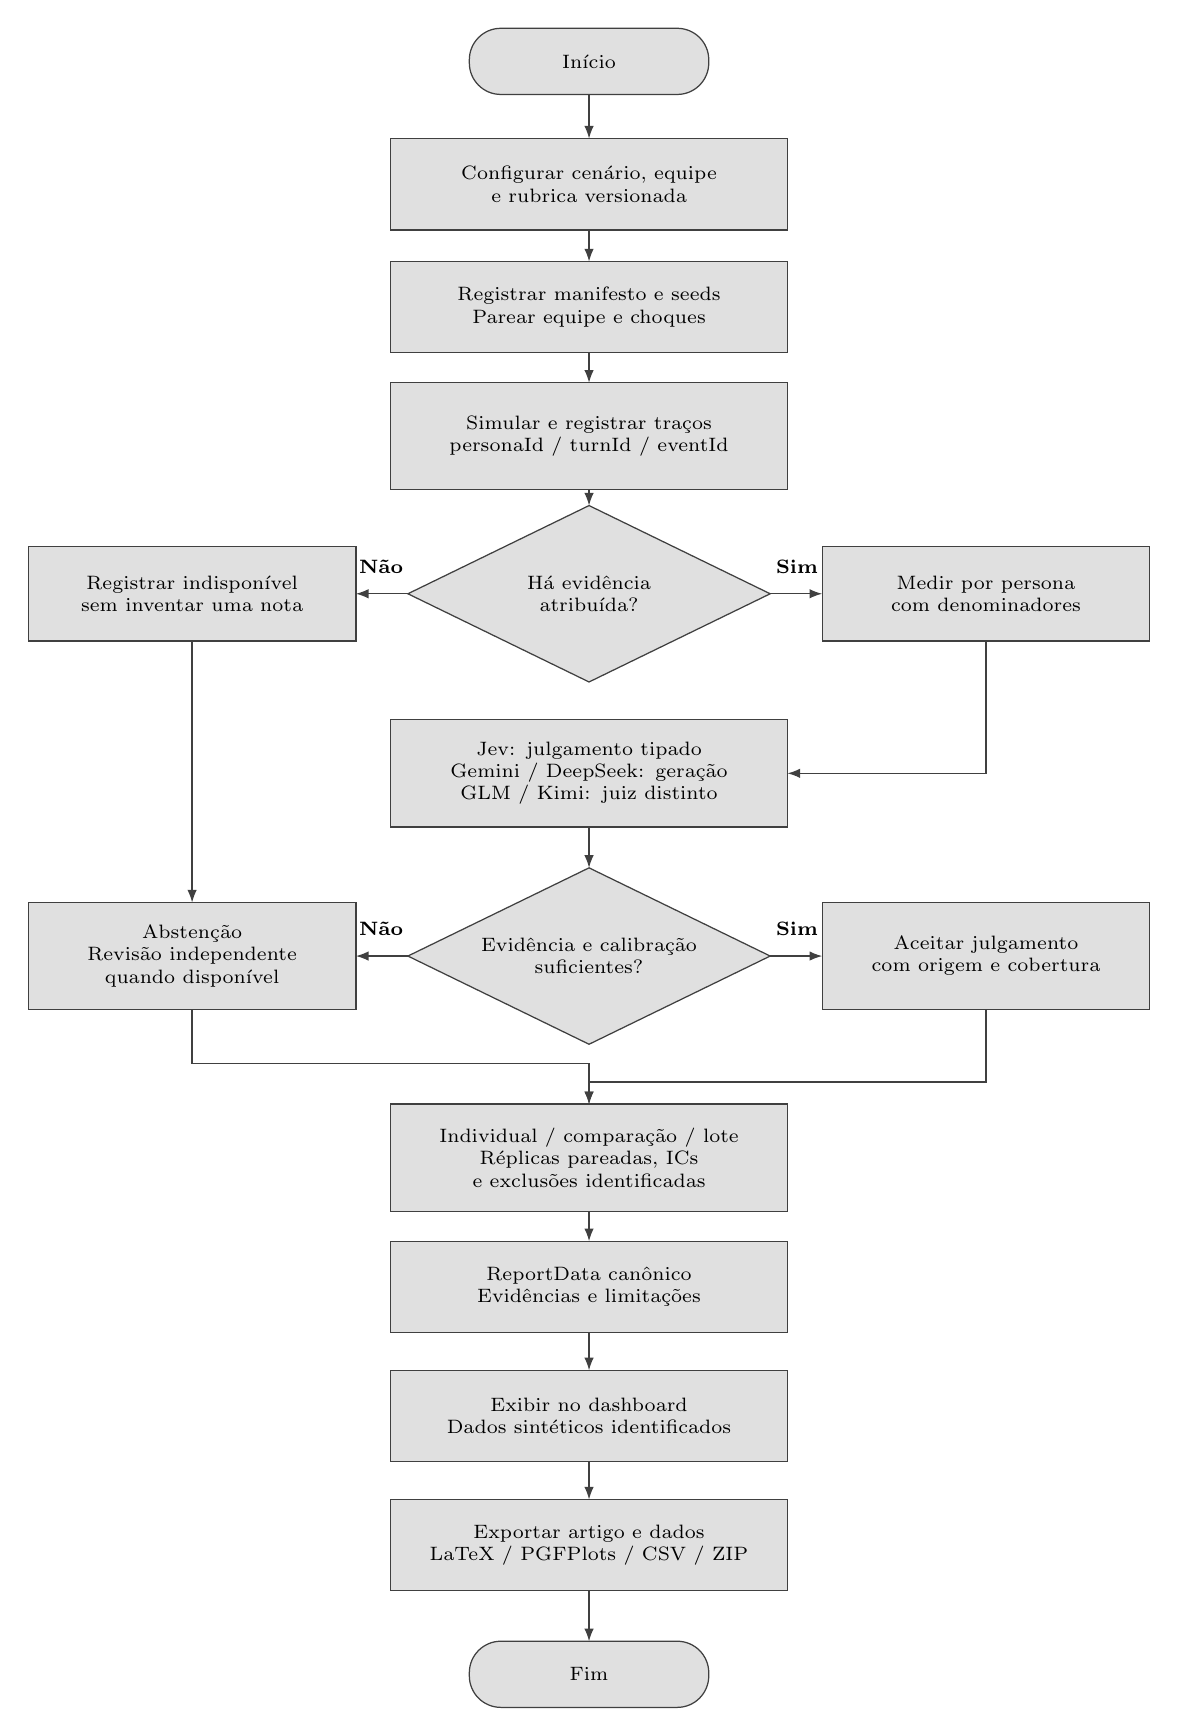
\begin{tikzpicture}[x=.02cm,y=-.02cm]
\draw[-{Latex[length=1.6mm]},draw=black!75,line width=.45pt] (380,49) -- (380,77);
\draw[-{Latex[length=1.6mm]},draw=black!75,line width=.45pt] (380,135) -- (380,155);
\draw[-{Latex[length=1.6mm]},draw=black!75,line width=.45pt] (380,213) -- (380,232);
\draw[-{Latex[length=1.6mm]},draw=black!75,line width=.45pt] (380,300) -- (380,310);
\draw[-{Latex[length=1.6mm]},draw=black!75,line width=.45pt] (265,366) -- (232,366);
\node[font=\scriptsize\bfseries,inner sep=0pt] at (248,349) {Não};
\draw[-{Latex[length=1.6mm]},draw=black!75,line width=.45pt] (495,366) -- (528,366);
\node[font=\scriptsize\bfseries,inner sep=0pt] at (512,349) {Sim};
\draw[-{Latex[length=1.6mm]},draw=black!75,line width=.45pt] (128,396) -- (128,562);
\draw[-{Latex[length=1.6mm]},draw=black!75,line width=.45pt] (632,396) -- (632,480) -- (506,480);
\draw[-{Latex[length=1.6mm]},draw=black!75,line width=.45pt] (380,514) -- (380,540);
\draw[-{Latex[length=1.6mm]},draw=black!75,line width=.45pt] (265,596) -- (232,596);
\node[font=\scriptsize\bfseries,inner sep=0pt] at (248,579) {Não};
\draw[-{Latex[length=1.6mm]},draw=black!75,line width=.45pt] (495,596) -- (528,596);
\node[font=\scriptsize\bfseries,inner sep=0pt] at (512,579) {Sim};
\draw[-{Latex[length=1.6mm]},draw=black!75,line width=.45pt] (128,630) -- (128,664) -- (380,664) -- (380,690);
\draw[-{Latex[length=1.6mm]},draw=black!75,line width=.45pt] (632,630) -- (632,676) -- (380,676) -- (380,690);
\draw[-{Latex[length=1.6mm]},draw=black!75,line width=.45pt] (380,758) -- (380,777);
\draw[-{Latex[length=1.6mm]},draw=black!75,line width=.45pt] (380,835) -- (380,859);
\draw[-{Latex[length=1.6mm]},draw=black!75,line width=.45pt] (380,917) -- (380,941);
\draw[-{Latex[length=1.6mm]},draw=black!75,line width=.45pt] (380,999) -- (380,1031);
\filldraw[fill=black!12,draw=black!75,line width=.45pt,rounded corners=4mm] (304,7) rectangle (456,49);
\node[align=center,text width=2.84cm,font=\scriptsize,inner sep=0pt] at (380,28) {Início};
\filldraw[fill=black!12,draw=black!75,line width=.45pt] (254,77) rectangle (506,135);
\node[align=center,text width=4.84cm,font=\scriptsize,inner sep=0pt] at (380,106) {Configurar cenário, equipe\\e rubrica versionada};
\filldraw[fill=black!12,draw=black!75,line width=.45pt] (254,155) rectangle (506,213);
\node[align=center,text width=4.84cm,font=\scriptsize,inner sep=0pt] at (380,184) {Registrar manifesto e seeds\\Parear equipe e choques};
\filldraw[fill=black!12,draw=black!75,line width=.45pt] (254,232) rectangle (506,300);
\node[align=center,text width=4.84cm,font=\scriptsize,inner sep=0pt] at (380,266) {Simular e registrar traços\\personaId / turnId / eventId};
\filldraw[fill=black!12,draw=black!75,line width=.45pt] (380,310) -- (495,366) -- (380,422) -- (265,366) -- cycle;
\node[align=center,text width=3.85cm,font=\scriptsize,inner sep=0pt] at (380,366) {Há evidência\\atribuída?};
\filldraw[fill=black!12,draw=black!75,line width=.45pt] (24,336) rectangle (232,396);
\node[align=center,text width=3.96cm,font=\scriptsize,inner sep=0pt] at (128,366) {Registrar indisponível\\sem inventar uma nota};
\filldraw[fill=black!12,draw=black!75,line width=.45pt] (528,336) rectangle (736,396);
\node[align=center,text width=3.96cm,font=\scriptsize,inner sep=0pt] at (632,366) {Medir por persona\\com denominadores};
\filldraw[fill=black!12,draw=black!75,line width=.45pt] (254,446) rectangle (506,514);
\node[align=center,text width=4.84cm,font=\scriptsize,inner sep=0pt] at (380,480) {Jev: julgamento tipado\\Gemini / DeepSeek: geração\\GLM / Kimi: juiz distinto};
\filldraw[fill=black!12,draw=black!75,line width=.45pt] (380,540) -- (495,596) -- (380,652) -- (265,596) -- cycle;
\node[align=center,text width=3.85cm,font=\scriptsize,inner sep=0pt] at (380,596) {Evidência e calibração\\suficientes?};
\filldraw[fill=black!12,draw=black!75,line width=.45pt] (24,562) rectangle (232,630);
\node[align=center,text width=3.96cm,font=\scriptsize,inner sep=0pt] at (128,596) {Abstenção\\Revisão independente\\quando disponível};
\filldraw[fill=black!12,draw=black!75,line width=.45pt] (528,562) rectangle (736,630);
\node[align=center,text width=3.96cm,font=\scriptsize,inner sep=0pt] at (632,596) {Aceitar julgamento\\com origem e cobertura};
\filldraw[fill=black!12,draw=black!75,line width=.45pt] (254,690) rectangle (506,758);
\node[align=center,text width=4.84cm,font=\scriptsize,inner sep=0pt] at (380,724) {Individual / comparação / lote\\Réplicas pareadas, ICs\\e exclusões identificadas};
\filldraw[fill=black!12,draw=black!75,line width=.45pt] (254,777) rectangle (506,835);
\node[align=center,text width=4.84cm,font=\scriptsize,inner sep=0pt] at (380,806) {ReportData canônico\\Evidências e limitações};
\filldraw[fill=black!12,draw=black!75,line width=.45pt] (254,859) rectangle (506,917);
\node[align=center,text width=4.84cm,font=\scriptsize,inner sep=0pt] at (380,888) {Exibir no dashboard\\Dados sintéticos identificados};
\filldraw[fill=black!12,draw=black!75,line width=.45pt] (254,941) rectangle (506,999);
\node[align=center,text width=4.84cm,font=\scriptsize,inner sep=0pt] at (380,970) {Exportar artigo e dados\\LaTeX / PGFPlots / CSV / ZIP};
\filldraw[fill=black!12,draw=black!75,line width=.45pt,rounded corners=4mm] (304,1031) rectangle (456,1073);
\node[align=center,text width=2.84cm,font=\scriptsize,inner sep=0pt] at (380,1052) {Fim};
\end{tikzpicture}
\end{center}
\end{document}
